\documentclass[%
a4paper,
%twoside,
11pt
]{article}

% encoding, font, language
\usepackage[T1]{fontenc}
\usepackage[utf8]{inputenc}
\usepackage{lmodern}
\usepackage[english]{babel}

\usepackage{nicefrac}

\usepackage[
    % handwritten,
    nowarnings,
    %myconfig
]
{xcookybooky}

\DeclareRobustCommand{\textcelcius}{\ensuremath{^{\circ}\mathrm{C}}}


\setcounter{secnumdepth}{1}
\renewcommand*{\recipesection}[2][]
{%
    \subsection[#1]{#2}
}
\renewcommand{\subsectionmark}[1]
{% no implementation to display the section name instead
}


\usepackage{hyperref}    % must be the last package
\hypersetup{%
    pdfauthor            = {Magdalena Przybyła, Hubert Bereś},
    pdftitle             = {Bethan's and Hugh's cookbook},
    pdfstartview         = {FitV},
    pdfview              = {FitH},
    pdfpagemode          = {UseNone}, % Options; UseNone, UseOutlines
    bookmarksopen        = {true},
    pdfpagetransition    = {Glitter},
    colorlinks           = {true},
    linkcolor            = {black},
    urlcolor             = {blue},
    citecolor            = {black},
    filecolor            = {black},
}

\hbadness=10000	% Ignore underfull boxes

\begin{document}

\title{Bethan's and Hugh's cookbook}
\author{Magdalena Przybyła, Hubert Bereś}
\maketitle

\begin{abstract}
    Some initial blah blah.
\end{abstract}

\tableofcontents

\vspace{5em}

\section{Basic recipes}
A bit more of initial blah blah.
\begin{recipe}
    [% 
        preparationtime = {\unit[30]{min}},
        bakingtime = {\unit[40]{min}},
        portion = {\portion{5-6}},
        source = {jadlonomia.com: pasztet-warzywny-doskonay}
    ]
    {The perfect pâté}

    \introduction{%
        The ingredients last for about \unit[30x12]{cm} baking tray.
    }

    \ingredients{%
        1.5 glass & boiled milet \\
        1 glass & hazelnuts \\
        \unit[100]{ml} & vegetable oil \\
        2 & carrots \\
        2 & parsleys / parsnips \\
        1 & leek (only the white part) \\
        2 pieces & celery \\
        2 claws & garlic \\
        3 Tsp. & soy sauce \\
        2 grains & allspice \\
        2 leaves & bay leaf \\
        1 tsp. & marjoram \\
        1 tsp. & parsley (dried) \\
        0.5 tsp. & lovage \\
        0.5 tsp. & thyme \\
        a pinch & nutmeg \\
        & salt and pepper
    }

    \preparation{%
        \step Slice the leek thinly, fry on oil with the bay leafs and the allspice on small heat until soft.
        In meantime, peel and grate carrots and parsnip.
        Chop the celery into small cubes, chop the garlic.
        \step Take out the bay leaf and allspice, add the prepared vegetables and stew on small heat for 10-15 minutes until they are very soft.
        \step Put the cooked vegetables in a large bowl.
        Add the milet, nuts, remaining oil and all the spices.
        Blend everything into uniform paste.
        \step Fill a baking tray laid out with baking paper or lubricated with oil.
        Bake for 30-45 minutes at \unit[200]{\textcelcius} until the top is dark gold and crispy.
        Cool down for a couple of hours before slicing.
    }

    \hint{%
        To avoid wet bottom, strew a thick layer of breadcrumbs in the baking tray.
        You may use crushed hazelnuts as well.
    }

\end{recipe}
\newpage

\begin{recipe}
    [% 
        preparationtime = {\unit[0.5]{h}},
        bakingtime={\unit[1.5]{h}}
    ]
    {Beetroot carpaccio}

    \introduction{%
        Easy salad, perfect for hot summer garden party or as a starter before fancy dinner.
    }

    \ingredients{%
        4  & Beetroot (elongated ones are the best)\\
        & Feta cheese/goat cheese \\
        & Balsamic vinegar \\
        & Olive oil \\
        & Rocket \\
        & Pumpkin seed/pistachio
    }

    \preparation{%
        \step Cover washed raw beetroot in aluminium foil. Bake till tender (around 1-1.5h)
        \step Slices thinly. Sprinkle with olive oil, black pepper and balsamic vinegar.
        \step Scatter cheese, rocket and seeds. Add extra olive oil and balsamic vinegar.
    }

    \suggestion[Be efficient]
    {%
        It's a lot of faff to bake just a few beetroot. Instead, bake them when baking something different, as they're covered in foil, fragrances shouldn't permeate.
    }

\end{recipe}
\newpage

\begin{recipe}
[% 
    preparationtime = {\unit[0.5]{h}},
    bakingtime={\unit[0.5]{h}},
     portion = {\portion{4}}
]
{Risotto}
    
    \introduction{%
    	People still haven't figured out why exactly stirring makes risotto so delicious. There are a few theories, covering even spread of heat and increased 'leakage' of starch from rice grains. Regardless of the reason, bear in mind that stirring, keeping the broth hot at all time and adding it in small portions are essential! 
    }
    
    \ingredients{%
        350 g  & Risotto rice \\
        Bunch  & Asparagus \\
        3 & Red/yellow peppers \\
        1 & Red onion \\
        500 ml & Broth/stock \\
        200 ml& Apple cider \\
        & Cheese (Parmesan or mature cheddar) \\
        250 g & Pancetta (Smoked) 
    }
    
    \preparation{%
        \step Heat up broth and keep hot.
        \step Fry finely diced onion. Add rice and fry for 2-3 minutes.
        \step Add alternately broth and cider in small portions (ladle or two) at a time. Keep stirring rice. Add more liquid when previous portion almost absorbed. 
        \step In meantime roast peppers and fry asparagus (cut in 3 pieces) or fry both. Fry pancetta.
        \step Stir vegetable and pancetta in. Add cheese. 
       
    }
    
    \suggestion[]
    {%
      The larger the pan, the less stirring required as rice is heated more evenly. 
    }
    
\end{recipe}
\newpage

\begin{recipe}
    [% 
        preparationtime = {\unit[0.5]{h}},
        bakingtime={\unit[0.3]{h}}
    ]
    {Easy puff pastry}

    \ingredients{%
        1 sheet  & Puff pastry\\
        1/2 jar & Pesto rosso\\
        1/2 can & Sweetcorn\\
        1/2 & Cream cheese
    }

    \preparation{%
        \step Roll the puff pastry (rectangual shape). Spread evenly, sequentially cream cheese and pesto.
        \step Scatter sweetcorn and other ingredients (see the tip).
        \step Roll using the long end. Cut into ellipses.
        \step Bake till brown and puffed at \unit[180]{\textcelcius}.
    }

    \suggestion[Spice it up!]
    {%
        Add fried chorizo (fry without extra oil!) or sautéed mushrooms
    }

\end{recipe}
\newpage

\begin{recipe}
[% 
    preparationtime = {\unit[0.5]{h}},
    bakingtime={\unit[1]{h}},
    bakingtemperature={\protect\bakingtemperature{
       topbottomheat=\unit[195]{dC}},
    portion = {\portion{6-8}},
    source = {polish wisdom}
]
{Strawberry cake}
    
    
    \introduction{%
        \blindtext
    }
    
    \ingredients{%
        \textbf{Sponge}  & 
        5  & eggs\\
        \unit[3/4]{c} & Sugar\\
        \unit[3/4]{c} & Flour\\
        \unit[1/4]{c} & Starch (Potato or corn)\\
        \textbf{Cream} & 
        \unit[3]{c} & Milk\\
        \unit[3/4]{c} & Sugar\\
        \unit[4]{tbs} & Flour (heaped spoonful )\\
        \unit[4]{tbs} & Starch (heaped spoonful)\\
        \unit[150-250]{g} & Butter\\
        1 & Egg yolk\\
    }
    
    \preparation{%
        \step All ingredients for sponge must be at room temperature. Beat whites until stiff. While still beating, add sugar (one spoon at the time). Then egg yolks (one at the time, still beating gently).   
        \step Add sifted flour. \underline{Don't beat.} Gently mix with a spatula.
        \step Line the cake tin with parchment (only bottom), don't grease sides. Fill with batter. Bake at 160-170$^\circle$C for 35-40min. 
        \step Boil 2/3 milk and sugar up. In a cup or high blender dish mix (with fork or a beater) flour, yolk and remaining milk. When sugar/milk liquid is boiling, add flour/milk and stir vigorously for about 2 min. Remove from heating and continue stirring. 
        \step Cool the blancmange (step 4). Cream butter and mix with blancmange (add in small portions).
        \step Sandwich the sponge and decorate with fresh fruit!  
    }
    
    \suggestion[Spice it up!]
    {%
      To make chocolate cream, add cocoa powder to milk-flour mixture. 
    }
    
   
    
    \tipp{%
        Drop hot sponge in the tin on the kitchen bench/floor from 30cm. Trust me, it will keep the cake fluffier.
    }
    
\end{recipe}
\newpage

\begin{recipe}
    [% 
        preparationtime = {\unit[0.5]{h}},
        bakingtime={\unit[1.5]{h}}
    ]
    {Beetroot carpaccio}

    \introduction{%
        Easy salad, perfect for hot summer garden party or as a starter before fancy dinner.
    }

    \ingredients{%
        4  & Beetroot (elongated ones are the best)\\
        & Feta cheese/goat cheese \\
        & Balsamic vinegar \\
        & Olive oil \\
        & Rocket \\
        & Pumpkin seed/pistachio
    }

    \preparation{%
        \step Cover washed raw beetroot in aluminium foil. Bake till tender (around 1-1.5h)
        \step Slices thinly. Sprinkle with olive oil, black pepper and balsamic vinegar.
        \step Scatter cheese, rocket and seeds. Add extra olive oil and balsamic vinegar.
    }

    \suggestion[Be efficient]
    {%
        It's a lot of faff to bake just a few beetroot. Instead, bake them when baking something different, as they're covered in foil, fragrances shouldn't permeate.
    }

\end{recipe}
\newpage
\begin{recipe}
[% 
    preparationtime = {\unit[0.5]{h}},
    bakingtime={\unit[0.5]{h}},
    portion = {\portion{4}}
]
{Roast vegetables lunch}
    
    \ingredients{%
        1 & Bitternut squash \\
        2 & Apple (something like Reinette or White Transparent) \\
        3 & Peppers (red-yellow)\\
        1 & Red onion\\
         & Oil\\
        	& Smoked paprika\\
      & Paprika \\
        	& Chilli\\
         & Cinnamon  \\
         & Cumin \\
         & Coriander \\
       1 tbs. & Honey \\
        2 tbs. & Vinegar (eg. apple) or lemon juice
    }
    
    \preparation{%
        \step Cut pumpkin into small pieces, peppers into big squares, chop apples and cut onion into eights.
        \step Toss vegetable in oil and spices.
        \step Bake for about 30 min, stir from time to time.  
        \step In meantime cook the base - some grain - pearl barley, buckwheat or simply rice. 

    }
 
    \hint{%
        If you need something more filling, add a can of chickpea. 
    }
    
\end{recipe}
\newpage
% Complete recipe example
\begin{recipe}
[% 
    preparationtime = {\unit[0.5]{h}},
    portion = {\portion{4-5}},
]
{Thai soup}
  
    \ingredients{%
        2 cans & Coconut milk \\
        \unit[300-400]{ml} 	& Broth \\
        \unit[200]{g} & Peeled prawns \\
        & Baby corns \\
        & Mangetouts \\
        & Udon noodles \\
        & Dumplings \\
        & Bean sprouts \\
        & Spring onions \\
        & Ginger \\
        & Garlic \\
        & Lemon grass \\
        & Coriander (leaves and powder) \\
        & Cumin \\
        & Chilli \\
        & Curry powder/green curry paste \\
        & Lime
    }
    
    \preparation{%
        \step Fry grated/finely chopped ginger, garlic and spices. 
        \step Add coconut milk and broth; heat up.
        \step Add mangetouts, baby corns and noodles and dumplings (depending on dumplings, may need to add them later, so they're not overcooked)
        \step In meantime fry prawns on high heat.
        \step Add prawns, bean sprouts, lime juice and green onions to the soup.
    }
    
 
    
    \hint{%
        You can add any noodles you like, skip dumplings, change vegetable, add tofu... be imaginative! 
    }
    
\end{recipe}
\newpage
\begin{recipe}
    [% 
        preparationtime = {\unit[0.5]{h}},
        portion = {\portion{4-5}}
    ]
    {Cauliflower soup}
    \introduction{%
        Flavour of my childhood... It's such a simple but dainty creamy soup. Serve with fresh crusty bread.
    }

    \ingredients{%
        1 & Cauliflower \\
        2 & Carrots \\
        5 & Potato \\
        1 & Onion \\
        \unit[1.5]{l} & Broth \\
        \unit[200]{g} & Sour cream \\
        & Dill
    }

    \preparation{%
        \step Fry diced onion. Add chopped carrot and potatoes. Fry for 5-7 min.
        \step Pour hot broth in. Add florets of cauliflower. Cook till tender (about 20 min).
        \step Add dill (and chives).
        \step Mix sour cream with a few spoon of hot soup (so it doesn't curdle) and add to the pot of soup, stir well.
    }

\end{recipe}
\newpage
% Complete recipe example
\begin{recipe}
[% 
    preparationtime = {\unit[0.5]{h}},
    portion = {\portion{3-4}},
    bakingtime={\unit[0.5]{h}},
   
]
{Tart with beetroot and goat cheese}
    
    
  
    \ingredients{%
    	 & Puff pastry\\
       3 & Cooked/baked beetroot\\
       \unit[200]{g} 	& Goat cheese \\
        4 & Eggs\\
        \unit[200]{ml} & Sour cream \\
        1 tbs. & Flour \\
        & Thyme\\
        & Balsamic vinegar 
     
    }
    
    \preparation{%
        \step Mix eggs, cream, flour and spices.  
        \step Slice beetroot and goat cheese.
        \step Line oven dish with puff pastry, make a few holes with a fork. Blind bake for 5 min.
        \step Layer beetroot, then cheese. Pour over egg mixture. \underline{Bake for 25-30 min at \unit[180]{\textcelcius}.}
        \step  Sprinkle with balsamic vinegar.
       
    }
    
 
    
    
\end{recipe}
\newpage
% Complete recipe example
\begin{recipe}
[% 
    preparationtime = {\unit[0.5]{h}},
    portion = {\portion{4}},
    bakingtime={\unit[0.5]{h}}
]
{Curry with sweet potatoes and butternut squash}
    
    
  
    \ingredients{%
        1 & Onion \\
        1 & Sweet potato \\
        1 & Butternut squash \\
        1 can & Tomatoes
        2 c. & Kale \\
        1-2 cans & Chickpea \\
        1 can & Coconut milk \\
        & \\
        & Curry powder \\
        & Turmeric \\
        & Coriander \\
        & Cumin \\
        & Garam Masala \\
        & Cinnamon \\
        & Cloves
    }
    
    \preparation{%
        \step Dice onion, chop up sweet potatoe and butternut squash
       \step  Fry onion with spices.
        \step Line oven dish with puff pastry, make a few holes with a fork. Blind bake for 5 min.
        \step Layer beetroot, then cheese. Pour over egg mixture. Bake for 25-30 min.
        \step  Sprinkle with balsamic vinegar.
    }

\end{recipe}
\newpage
% Complete recipe example
\begin{recipe}
[% 
    preparationtime = {\unit[0.5]{h}},
    portion = {\portion{3-4}},
    bakingtime={\unit[40]{min}}
]
{Asparagus tart}

    \ingredients{%
        \unit [200]{g} & Flour \\
        \unit [120]{g} &Butter \\
        1 & Egg \\
        1 ts. & salt \\
        & \\
        Bunch & Asparagus \\
        \unit [200]{ml} & Sour cream \\
        2 & Egg \\
        1 tbs. & Flour \\
        & Nutmeg \\
        & Salt\&pepper \\
        & Thyme
    		}

    \preparation{%
       \step Knead shortcrust pastry. Cover with cling film and refrigerate for 30min. 
       \step Remove lignified ends of asparagus. Wash and cook for 4 min (water shall not cover heads).
       \step Beat eggs, mix with sour cream, flour and spices.
       \step Grease baking dish with butter, line with pastry (roll circle bigger than the dish and transport it on roller). Lay asparagus and pour the egg mix over.
       \step Bake at for about 40 min at \unit[160-170]{\textcelcius}.
             
    }

\end{recipe}
\newpage
\begin{recipe}
    [% 
        preparationtime = {\unit[15]{min}},
        portion = {\portion{2}},
        bakingtime = {\unit[15]{min}}
    ]
    {Fruity omelette}

    \ingredients{%
        5 & Egg \\
        \nicefrac{1}{2} c. & Flour \\
        1 ts. & Baking powder \\
        \nicefrac{1}{4} c. & Sugar \\
        \nicefrac{1}{4} c. & Milk/water \\
        & Raspberries \\
        \nicefrac{1}{2} c. & Yoghurt/quark to serve with
    }

    \preparation{%
        \step Beat eggs with milk.
        Mix well with flour, baking powder and sugar.
        \step Gently stir raspberries in.
        \step Pour the mixture on a preheated frying pan.
        \step Fry for 4 min on medium heat, after that cover the pan and leave for another 4 min.
        \step Flip the omelette and repeat step 4.
        \step Serve with yoghurt, honey, nuts... whatever you fancy!

    }

    \hint{%
        You can also add a little bit of yoghurt or quark to the batter, as weel as some spices - ginger, cinnamon...
    }

\end{recipe}
\newpage
\begin{recipe}
    [% 
        preparationtime = {\unit[15]{min}},
        bakingtime = {\unit[30]{min}}
    ]
    {Granola}

    \introduction{%
        There's nothing better than a quick home-made breakfast. Granola is a great base - add seasonal fruit, yoghurt or milk and bob's your uncle, delicious meal is ready.
    }

    \ingredients{%
        2.5 c. & Regular rolled oats \\
        0.5 c. & Walnuts \\
        0.5 c. & Hazelnuts \\
        0.5 c. & Sunflower seeds \\
        0.5 c. & Honey \\
        0.25 c. & Oil \\
        2 ts. & Cinnamon \\
        2 ts. & Ginger \\
        Pinch & Salt
    }

    \preparation{%
        \step Heat honey and oil slightly, just so you can mix them. Add spices and salt.
        \step In a big bowl, mix oats and nuts. Add honey/oil mixture and cover everything evenly.
        \step Transfer granola to big and flat baking tray, spread out evenly. \underline{Bake at  \unit[180]{\textcelcius} for 20-30 min}, mix with spatula every 5 min and keep an eye not to burn the granola!
        \step Store in an airtight jar.
    }

    \hint{%
        When the granola cooled down, you can add chopped dried fruit - eg. apricots and cranberry. You can also add some coca powder to honey - this granola will be happy when accompanied by dried cherries. Use different flakes (check out millet flakes or barley flakes - you can find them in polish shops certainly). You can also add some orange juice to honey. Chocolate chips, coconut flakes, etc...  There's so much room for imagination!
    }

\end{recipe}
\newpage
% Complete recipe example
\begin{recipe}
[% 
    preparationtime = {\unit[15]{min}},
    bakingtime={\unit[50]{min}}
]
{Banana bread with blueberries}
 \introduction{%
	Forgot about bananas? This recipe will save them. Perfect for afternoon tea or even breakfast. Simple sweet treat!  
}

    \ingredients{%
    	4-5 & Ripe bananas \\
        0.25 c. & Oil \\
        0.25 c. & Peanut butter \\
        0.25 c. & Milk \\
        2 handf. & Blueberries (fresh or frozen) \\
        & \\
        2 c. & Flour \\
        0.5 c. & Sugar \\
        1.5 ts. & Baking powder \\
        2 handf. & Desiccated coconut \\
        1 handf. & Chopped nuts \\
        & Spices (cinnamon, ginger, cardamom)
       }

    \preparation{%
       \step Turn bananas into purée (blend or use fork), mix with all other 'wet' ingredients. 
       \step Mix all dry ingredients in a separate bowl. Add in small portions and mix into the wet ingredients.
       \step Add blueberries.
       \step Bake for about 50 min at \unit[180]{\textcelcius} in a small rectangular tin lined with baking paper.
    }

 \hint{%
	You can skip blueberries and add some chocolate chips.
}

\end{recipe}
\newpage
\begin{recipe}
    [% 
        preparationtime = {\unit[5]{min}},
        bakingtime = {\unit[20]{min}}
    ]
    {Rhubarb compote}

    \introduction{%
        When you fancy something nice to drink but don't want to reach for rich in sugar juices - go for compote!
        You can prepare compote from pretty much any seasonal fruit.
        My favourite one is rhubarb compote (M.), then plum and White Transparent apple (not sure if you can get theme here...).
    }

    \ingredients{%
        800 & Rhubarb \\
        2 l & Water \\
        & Sugar \\
        hfl. & Mint \\
        hfl. & Berries
    }

    \preparation{%
        \step Cur rhubarb into 3-4 cm long pieces.
        Fry with a little bit of sugar.

        \step Add 2 l of water and simmer for about 15 min.
        After 10 min, add berries and mint.

        \step Add more sugar if needed.
    }

\end{recipe}
\newpage
\begin{recipe}
    [% 
        preparationtime = {\unit[15]{min}},
        portion = {\portion{4}},
        bakingtime = {\unit[30]{min}}
    ]
    {Rhubarb crumble}

    \introduction{%
        There are three reasons why I love crumbles: preparation is super quick;
        no wheat; little sugar yet is very sweet due to fruit.
    }

    \ingredients{%
        600-800 g & Rhubarb \\
        5 & Apricots \\
        2 hfl. & Berries \\
        2 hfl. & Blueberries (fresh or frozen) \\
        & \\
        100 g. & Butter \\
        \nicefrac{1}{2} c. & Sugar \\
        1~\nicefrac{1}{2} c. & Oat flakes \\
        3 tbs. & Coconut milk powder \\
        1 tbs. & Ginger \\
        \nicefrac{1}{4} ts. & Salt
    }

    \preparation{%
        \step Cut rhubarb into 2-3 cm long pieces, apricots into quarters.
        Mix with berries in an oven dish/tin.


        \step In a hand blender s-shaped knife container (or using your hands) mix all ingredients for crumble topping.
        Add more fat/oats if needed


        \step Cover fruit with crumble topping. \underline{Bake at}
        \underline{\unit[180-200]{\textcelcius} for 20-30 min} till brown.
    }

    \hint{%
        Serve with ice cream or clotted cream.
    }

\end{recipe}


\begin{figure}[h]
    \centering
    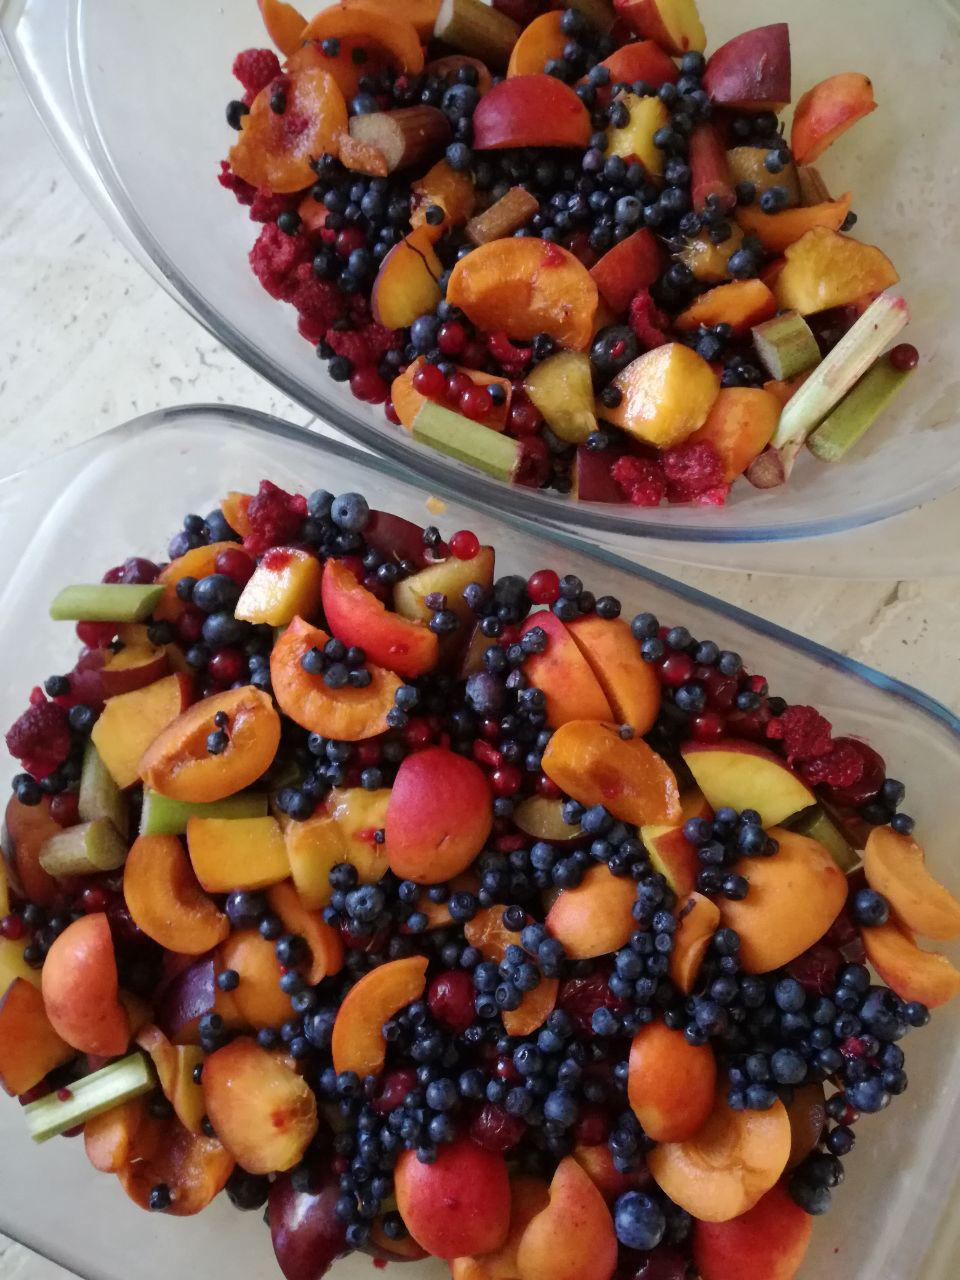
\includegraphics[width=12cm]{pic/crumble}
\end{figure}

\newpage
\begin{recipe}
    [% 
        preparationtime = {\unit[20]{min}},
        bakingtime = {\unit[15]{min}}
    ]
    {Chickpea cookies}

    \introduction{%
        I know that for Bethan 'a treat is a treat' but I believe that there are plenty of puddings and snacks that are not only scrumptious but also carry some nutrients. Incorporating pulses and vegetable to desserts in an endless adventure.
    }

    \ingredients{%
        1 can & Chickpea \\
        0.5 c. & Peanut butter \\
        0.25 c. & Honey \\
        2 heaping tbs. & Flour \\
        50 g & Chocolate, chopped into small pieces \\
        1 ts. & Cinnamon \\
        0.5 ts. & Baking powder }

    \preparation{%
        \step With the help of a blender, mix all ingredients apart for flour and chocolate.

        \step When chickpea is well mashed, add flour and continue blending. Mix chocolate in (use spatula).

        \step Using a spoon form cookies (line baking tray with baking paper) \underline{Bake at \unit[180]{\textcelcius}} \underline{for 15 min till brown.}
    }

\end{recipe}
\newpage
% Complete recipe example
\begin{recipe}
[% 
    preparationtime = {\unit[10]{min}},
    portion = {\portion{2}},
    bakingtime={\unit[15]{min}}
]
{Quick chicken curry soup}

\introduction{%
	It may be the only recipe containing meat, well one can give someone only what he posses... This soup is a tasty relict of the first year at uni and Sunday lunches in Cryfield ;) 
}

    \ingredients{%
    	400 ml & Broth/water \\
    	1-2  & Chicken breast \\
        0.5 c. & Red lentil \\
        2 & Carrots, sliced/diced \\
        1 & Onion, diced \\
        2cm & Ginger, diced \\
        3 & Garlic cloves, diced/pressed \\
        1 can & Chopped tomatoes \\
        1 can & Coconut milk \\
        & Curry powder \\
        & Garam masala \\
        & Cinnamon 
     }

    \preparation{%
       \step Cut chicken into relatively small pieces. Fry with onion, garlic, ginger and spices.   
       \step When chicken is slightly brown, pour broth, canned tomatoes. Add lentils, carrot and salt.
       \step When carrot and lentil is almost tender, add coconut milk, and boil for a few minutes without a lid. Add more spices if needed.
       \step \underline{Serve with naan bread.}
      }

\end{recipe}

\section{Fancy recipes}
A bit more involved.

% Complete recipe example
\begin{recipe}
[% 
    preparationtime = {\unit[1]{h}},
    bakingtime={\unit[1]{h}},
    portion = {\portion{4-5}}
]
{Lasagne with pumpkin and millet}
    
    \ingredients{%
        \unit[2]{c} & Pumpkin purée \\
        \unit[3/4]{c} & Millet \\
        \unit[200]{ml} & Cream \\
        Handful & Capers \\
        Handful & Dried tomatoes \\
        & Sage \\
        Box	& Lasagne sheets \\
        \textbf{Sauce} & \\
        2 cans & Tomatoes \\
        \unit[400]{ml} & Passata \\
        1 & Onion \\
        & Smoked paprika \\
        & Balsamic vinegar \\
        & \\
        & Cheese for topping - mozzarella or grated cheddar
    }
    
    \preparation{%
        \step Rinse millet with boiling water. Add 1.5 c of water, salt and cook at small heat till millet absorbed all liquid. If still not tender, add more water and cook till tender. When cooking millet, leave it alone, don't stir it, don't uncover it etc. 
        \step Fry onion, add all sauce ingredients and simmer for as long as you can.
        \step Mix with blender cooked millet, pumpkin purée and remaining filling ingredients apart for capers and dried tomatoes. Add capers and chopped dried tomatoes.  
        \step In high oven dish layer alternately sauce, lasagne sheets, pumpkin filling and lasagne sheet. End with sauce, add cheese on the top.
        \step Bake for about an 1h (check if pasta is tender).
    }
    
    \suggestion[]
    {%
       You can also prepare béchamel sauce and either alternate it with tomato sauce or replace. 
    }
    
    
    \hint{%
        For extra umami flavour, add yeast flakes to the pumpkin filling or cook millet in broth. 
    }
    
\end{recipe}
\newpage
\begin{recipe}
    [% 
        preparationtime = {\unit[1.5]{h}},
        portion = {\portion{4}},
        bakingtime = {\unit[0.5]{min}}
    ]
    {Polish croquette with spinach and feta cheese}

    \ingredients[20]{%
        2 c. & Flour \\
        4 & Eggs \\
        2 c. & Milk \\
        1.5 c. & Water \\
        pinch & Salt \\
        2 tbs. & Oil \\
        & \\
        800 g & Spinach \\
        5 & Garlic cloves \\
        200 g & Feta cheese \\
        & Nutmeg \\
        & \\
        & Breadcrumbs \\
        & Beaten egg
    }

    \preparation{%
        \step Mix all ingredients for crepes batter. Fry crepes on a greased frying pan.

        \step Fry spinach, nutmeg and garlic till most of the water from spinach evaporates. Then add crushed feta cheese and mix well.

        \step Croquette folding - see picture.

        \begin{figure}[!h]
            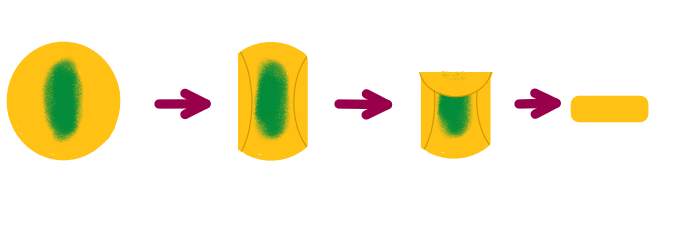
\includegraphics[width=.6\linewidth]{krokiety}
        \end{figure}

        \step Folded croquettes dip in beaten egg (with salt and pepper) and then cover with breadcrumbs. Fry till brown (you'll need relatively lots of oil).
    }

    \suggestion{%
        Now try different fillings. Maybe mushroom, pepper and cheddar?
    }

\end{recipe}
\newpage
% Complete recipe example
\begin{recipe}
[% 
    preparationtime = {\unit[0.5]{h}},
    portion = {\portion{3-4}},
    bakingtime={\unit[0.5]{h}}
]
{Carrot \textit{kopytka}}
    
    
  
    \ingredients{%
    	\unit[500]{g} 	& Carrot purée \\
    	\unit[200]{g} 	& Starch \\
    	\unit[200]{g} 	& Corn flour \\
    	2 tbs. & Yeast flakes \\
        & Nutmeg \\
       
        \textbf{Sauce} & 
        5 & Garlic cloves \\
        2 tbs. & Tahini \\
        2 tbs. & Soy sauce \\
        1/2 & Lime\\
        2 tbs. & Sesame oil \\
        1 ts. & Coriander \\
        1 ts. & Cumin \\
        
     
    }
    
    \preparation{%
        \step  Boil 5l of water.
        \step Knead all ingredients for dough. Roll and cut into small rods (see picture). 
        \step Cook \textit{kopytka} in hot water till tender (about 3 min from the moment when they started floating - as opposed to stay at the bottom of the pot).
        \step Heat frying pan with some oil. Add all ingredients of the sauce (do it in chunks if you're not going to fit all of the \textit{kopytka} at once).
        \step  Fry \textit{kopytka} and covered in sauce. Serve with greens. 
       
    }
    
 
    
    
\end{recipe}
\newpage
% Complete recipe example
\begin{recipe}
[% 
    preparationtime = {\unit[1]{h}},
    portion = {\portion{2}},
    bakingtime={\unit[40]{min}}
]
{Roast pepper and cheese galette}
    
    \introduction{%
    	Whenever I think about fancy dinner (supper?), I reach for stuffed pastry. Ladies and gentlemen, tonight we're serving French galette!
    }
    
  
    \ingredients{%
    	\unit[200]{g} & Flour \\
       1/4 tbs. & Salt\\
       \unit[100]{g} 	& Butter \\
        \unit[100]{g}  & Sour cream \\
       \textbf{Filling }&  \\
       2 & Pepper \\
       1 & Garlic clove \\
       \unit[100]{g} 	& Ricotta \\
       \unit[50]{g} 	& Cheese (eg. Grana Padano) \\
       \unit[50]{g} 	& Mozzarella \\
        & Fresh basil
     }
    
    \preparation{%
        \step Mix flour, salt and cold butter. Add sour cream and quickly knead the dough. If needed, add spoon or two of cold water. \underline{Cover with foil and leave in the fridge for an hour.}
        \step Roast slices of pepper (30 min, \unit[200]{\textcelcius})
        \step In a bowl, mix garlic and olive oil, salt and pepper to taste.
        \step On bench covered with flour, stretch the dough to form a circle, place it on parchment. In the middle (leaving about 5 cm edge) spread ricotta, mozzarella and Grana Padano. Place pepper on the cheese, starting with the outer edge of the cheesy filling.  
        \step  Wrap free edges towards the centre (see picture).
        \step Bake for 30-40 min.
        \step Garnish with basil leaves. 
       
    }
    
  \hint{%
 	If the dough is very gluey, wet your hands for easier handling. }
    
\end{recipe}

\end{document} 